\chapter{How to Show, Not Tell}

この講義には、ふつうの意味での数学はほとんどない。だが、形式的な背骨はたしかにある。私たちは、散文をひとつの inferential system として考えるよう求められる。読者に結論をそのまま手渡すのか、それとも、その結論を読者自身が回収できるような evidence を手渡すのか。講義はかなり注意深く展開される。わざと悪く書かれた冒頭の passage が問題を作り、一連の concessions がこの lesson を mere slogan にしてしまうのを防ぎ、そこから六つの principles が craft を sharpen していく。私たちはその順序に従おう。というのも、この argument は、その個々の claims と同じくらい、その progression に依存しているからである。

\begin{remark}
ここには文字どおりに transcription すべき黒板数学はない。以下の displayed equations は editorial schemata である。講義の logic を compactify しているが、screen 上に symbolic formalism が現れたことを示唆するものではない。
\end{remark}

\section{冒頭の失敗}

講義は definition から始まらない。失敗から始まる。私たちは wilderness の passage を与えられる。そこでは少女が afraid であると言われ、sounds が frightening であると言われ、ground が guardian のように感じられると言われる。大事なことはすべて告知されている。だが、触知できるものはほとんど作られていない。

これは、正しい pedagogical opening である。講師は、その弱さに名前を与える前に、まずその weakness を感じさせたいのだ。prose は fear を dramatize せずに名指しし、atmosphere を create せずに名指ししている。私たちは、感覚的あるいは narrative な pressure によって justify されるべき emotional verdicts を、その justification なしに与えられているのである。

\subsection{Question \& Answer}

講義は立ち止まり、この章全体を支配する問いを発する。

What is wrong with this picture?

まずいのは、この passage に emotion words が含まれていることではない。問題は、この passage が evidence を供給する前に、conclusions を供給してしまっていることにある。fear は enact されずに assert されている。safety は earn されずに assert されている。scene がそうした feelings を避けがたいものにするべき、まさにその地点で、読者は何を think し、何を feel すべきかを told されてしまうのだ。

\begin{definition}
この講義の意味での \emph{telling} とは、結論、summary、trait、emotion を直接に述べることであり、\emph{showing} とは、そこから同じ結論が infer できるような dramatic、sensory、behavioral、あるいは perspectival な evidence を与えることである。
\end{definition}

K.\ M.\ Weiland の compact な distinction は、この講義に最初の clean な axis を与える。
\begin{align}
\text{showing} &= \text{dramatizing},\\
\text{telling} &= \text{summarizing}.
\end{align}

これはすでに、よくある confusion に対するひとつの correction である。summary 自体が enemy なのではない。unsupported な summary が enemy なのである。この講義は残りの時間を、その summary が有用な work をしているときと、scene を早々に閉じてしまっているときとを tell することに費やす。

\section{showing、telling、そして読者の仕事}

problem を sharply に提起したあとで、講義はすぐに rule を soften する。telling は、本質的に bad なものではない。もし passing な facts、時間の経過、routine な motion の一つひとつをすべて show しようとしたら、fiction は swollen で shapeless なものになってしまう。stories には compression が必要である。bridges が必要である。fully inhabited な moments と同じくらい、broad sweeps も必要なのである。

だからこそ、The Secret Garden の example がここに現れる。Mary Lennox は disagreeable-looking な child であり、しばしば ill であったと私たちは told される。だが prose は verdict で止まらない。thin face、thin body、light hair、sour expression へとただちに move する。summary は proof に anchoring されている。これが、この講義における legitimate な blend の model である。

講義の central logic は、図式的には
\begin{equation}
\text{concrete detail} \leadsto \text{reader inference} \leadsto \text{emotion or judgment}.
\end{equation}
と書ける。

ここで Andrew Stanton の storytelling metaphor が有用になる。transcript はやや garbled だが、secure な idea は明らかである。もし audience の active participation が欲しいなら、``4'' を与えてはならない。``2+2'' を与え、最後の一歩は audience 自身に perform させるべきなのだ。
\begin{equation}
2+2 \to \text{audience inference}, \qquad 4 \to \text{premature closure}.
\end{equation}

講義は insist する。これは decorative な advice ではない。読者は work をしたがる。ただし、その work が experience の内部に artfully hidden されているかぎりにおいて、である。彼らは deduce し、complete し、discover したがる。その意味で、showing とは、organized incompleteness の discipline である。scene の pressure のもとで読者自身がそこへ arrive できるように、私たちは final label を omit するのである。

\begin{figure}[h]
\centering
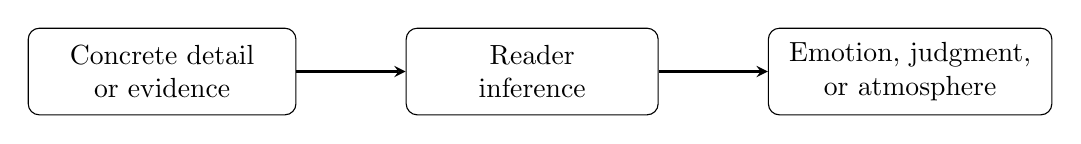
\begin{tikzpicture}[>=stealth]
\node[draw, rectangle, rounded corners, minimum width=3.4cm, minimum height=1.1cm, align=center] (a) at (0,0) {Concrete detail\\or evidence};
\node[draw, rectangle, rounded corners, minimum width=3.2cm, minimum height=1.1cm, align=center] (b) at (4.7,0) {Reader\\inference};
\node[draw, rectangle, rounded corners, minimum width=3.6cm, minimum height=1.1cm, align=center] (c) at (9.5,0) {Emotion, judgment,\\or atmosphere};
\draw[->, thick] (a) -- (b);
\draw[->, thick] (b) -- (c);
\end{tikzpicture}
\caption{講義の基本的な inferential pipeline。私たちは verdict に名前をつけるところから始めるのではない。verdict がほとんど inevitable になるような evidence を供給するところから始める。}
\end{figure}

ここから講義は、その claim を broaden する。cinematic storytelling について真であることは、prose についても真である。meaning が pointed out されるときよりも、implied されるときのほうが、読者はより強く care する。だからこそ講義は一歩引き、この mantra がどこから来たのかを問うことができる。

\section{なぜこの mantra が存在するのか}

六つの principles へ向かう前に、講義は短い historical detour を挿入する。これは ornamental ではない。この rule がこれほどの force を持つ理由を説明してくれる。

講師は、この modern slogan を realism の tradition の中へ置く。ordinary life を、romanticized されたり rhetorically overmanaged に感じられたりしないだけの immediacy と honesty をもって render しようとする試みである。そこで Percy Lubbock が、この distinction を major に formalize した人物として持ち出される。彼の key thought は、fiction が art になるのは、story が shown されるべきものとして扱われ、それゆえ story 自身が tell しているかのように見えるときだ、ということである。

Janice Hardy の practical な restatement は、その literary history を workshop language へと translate し直す。line が character の thought、perception、あるいは pressure のように feel されるかぎり、私たちはたいてい safe である。それが scene を decode するために author が stepping in してくる sound に聞こえた瞬間、immersion は弱まる。

この実践的傾向は、次のように要約できる。
\begin{equation}
\text{authorial explanation} \downarrow \;\Longrightarrow\; \text{reader immersion} \uparrow.
\end{equation}

これは absolute law ではない。講義は後になって exposition と narration を proper place へ restore するだろう。だが、この detour は real target を明らかにする。問題は telling の existence ではない。author が visible になりすぎることなのである。しかもそれは、scene を読者に内側から live させたい、まさにその point においてである。

この larger motivation が置かれたことで、講義は実践的になる準備が整う。いまから、それは順に六つの guiding principles へ移る。

\section{evidence、concrete detail、そして sensory specificity}

最初の三つの principles は、自然な cluster を成している。どれも同じ question に、別々の角度から答えている。もし emotional あるいは descriptive な conclusion をただ assert しないのなら、その place に私たちは何を置くのか。

\subsection{verdict より先に evidence}

第一の move は、もっとも clean である。もし narrator が husband は kind-hearted だと言うなら、もし protagonist が friend は guilty だと believe するなら、もし line が Adam knew Gwen liked him と言うなら、講師は私たちに、結論のところで pause し、その ground を探すよう求める。そもそも、誰がそう think するに至ったのか。

講義で引用される thought-verb exercise も、同じ point を示している。revision のために、私たちは一時的に \emph{knew}、\emph{believed}、\emph{wanted}、\emph{realized}、\emph{imagined} のような verbs を distrust する。forbidden だからではない。それらがしばしば、本当の scene を hide してしまうからである。

\paragraph{Worked revision.} 講義の sample line は ``Adam knew Gwen liked him.'' である。repair は mysterious ではない。methodical なのである。
\begin{enumerate}
\item conclusion から始める。Adam knew Gwen liked him.
\item Adam が actually perceives しているものは何かを問う。
\item hidden judgment を、繰り返される locker での encounter、painted metal に残る heel mark、perfume の smell、warm な combination lock に置き換える。
\item 読者が Adam の conclusion に unaided に reach できるところで止める。
\end{enumerate}

図式的には、
\begin{align}
\text{``Adam knew Gwen liked him''}
&\xrightarrow{\text{revision}}
\text{locker} + \text{heel mark} + \text{perfume} + \text{warm lock}.
\end{align}

したがって第一 principle は、単に ``detail を足せ'' ではない。もっと exact である。conclusion を、その conclusion を license する evidence へ置き換えよ、ということなのだ。

\subsection{abstract から concrete へ}

第二 principle は、同じ logic を emotion words や evaluative adjectives に適用する。Harvey Chapman の example が、この仕事を efficiently に果たしている。Toby walked home happier than he had ever felt と言う代わりに、better version は、彼の face から離れない grin と、almost stumbling するほど buoyant な movement を与える。

これは一般的な revision rule として
\begin{equation}
\text{abstract label} \xrightarrow{\text{revision}} \text{observable evidence}.
\end{equation}
と書ける。

講義の substitutions のいくつかは、この pattern を示している。
\begin{align}
\text{happy}
&\xrightarrow{\text{showing}}
\text{goofy grin} + \text{springing movement},\\
\text{eerie}
&\xrightarrow{\text{showing}}
\text{長く死んだ children の cries で humming する forest}.
\end{align}

point は、abstraction がいつでも illegitimate だということではない。point は、abstract words はしばしば too soon に到来するということである。scene がまだ meaning を felt させていないうちに、その scene が何を mean するのかを tell してしまうのだ。講義の eerie-forest の example は、まさにその理由ゆえに useful である。``The dark forest felt eerie'' は false ではない。ただ weak なのである。revised line は、その adjective に argument を向けるのではない。それを earn するのである。

\subsection{Question \& Answer}

私たちは、なお abstraction の中で書いているのだと、どうすれば分かるのか。

講義の operational な答えは simple である。camera がそれを see できるかを問え。もちろん、それは complete な test ではない。prose は smell、touch、taste、sound を invoke することもできるからだ。だが、first filter としては強い。camera がそれを see できないなら、sensory evidence がいったい何か、実際に何か supplied されているのかを問うべきである。

これがそのまま、第三の schematic rule へ直結する。
\begin{equation}
\text{cause statement} \xrightarrow{\text{showing}} \text{visible or sensory effect}.
\end{equation}

Jerry Jenkins の examples は、ここで理想的である。
\begin{align}
\text{cold}
&\xrightarrow{\text{showing}}
\text{collar up} + \text{scarf tightened} + \text{hands in pockets} + \text{風から顔を背ける},\\
\text{blindness}
&\xrightarrow{\text{showing}}
\text{bench を探る white cane},\\
\text{late fall}
&\xrightarrow{\text{showing}}
\text{足元で crunch する leaves}.
\end{align}

これは、この講義でもっとも重要な局所的 derivations の一つである。cause に名前をつける代わりに、その trace を書くのだ。``it was cold'' の代わりに、cold が何をするかを show する。``it was late fall'' の代わりに、ground にその season を sound させるのである。

講義はそのあと、この point を visibility の外へ extend する。Delilah Dawson の market scene は、concrete になるから強くなるだけではない。sensorily であり locally concrete になるから強くなる。cinnamon、coffee、silken tassels、powdered saffron。scene は、その particulars が vivid であり、しかもその world に singular であるとき、より immersive になる。

最後に講師は、subtle な warning を加える。technically には visual であっても、details が too expected であれば、scene は inert でありうる。rainy funeral は clear かもしれないが、それでも stale でありうる。だからこそ講義は、Gail Carson Levine の advice に立ち止まる。scene が clich\'ed に feel されるなら、setting を変えるか、emotional angle を変えるか、あるいは expectation を break する local anomaly をひとつ導入せよ。この段階で私たちは、もはや abstraction を detail へ置き換えているだけではない。generic detail を、\emph{this} story に属する detail へ置き換えているのだ。

\section{stock な body language の先へ}

ここで講義は、重要な correction を行う。いったん writers が show せよと言われると、彼らはしばしば、もっとも手近な shorthand へ走る。clenched fists、crossed arms、gritted teeth、racing hearts、rolling stomachs。これらが useless だというわけではない。だが、overuse するのはとても easy である。

いま danger は、以前より precise である。earlier には、danger は bare abstraction だった。ここでの danger は、shallow な concreteness である。ある emotional charge を signal する visible sign ではあるが、その source について十分には tell してくれない visible sign なのだ。

\subsection{Question \& Answer}

body language だけで十分なのか。

ふつうは十分でない。それは \emph{何か} が起こっていることを indicate するかもしれない。だがしばしば、それが \emph{どんな種類の} ものなのかを communicate し損ねる。anger は、単一の stock gesture へ還元されると、frustration、humiliation、jealousy、panic、grief に似てしまうことがある。講義の point は、body language はしばしば compressed されすぎていて、それ alone では emotional nuance を carry しきれない、ということだ。

Robin Patchen の before-and-after の example は、この point を decisive にする。第一 version では、Mary は clock を見て、heart が chest から飛び出しそうになり、stomach が roll し、何かが wrong なのではないかと fear する。一見すると、これは showing のように見える。たしかに bodily reaction は見えるからだ。だが講師は、この scene はなお melodramatic で overexplained に feel されると insist する。body がすべての work をしていて、thought-process がほとんど存在しないのである。

revised version は、center of gravity を変える。sunlight が window から stream する。Mary は rested に目を覚ます。clock を見る。little Jane が一晩中眠っていたのだと realize する。そこで別の memory が入る。Billy である。action はほとんど即座に続く。彼女は covers を flip back し、robe を snatch し、doctor の reassurance を自分に repeat する。これによって emotion は contour を持つ。それは単なる alarm ではない。memory と denial の pressure の下にある alarm なのである。

講義はこれを、保存すべき因果連鎖へ compress する。
\begin{equation}
\text{thoughts} \to \text{emotions} \to \text{actions}.
\end{equation}

これはおそらく、この講義でもっとも clean な ``equation'' である。scene が emotionally thin に feel されるとき、どこを見るべきかを tell してくれるからだ。bodily shorthand へ too quickly に leap すると、その feeling に exact な shape を与える thought を skip してしまう。thought を restore すれば、そこから生じる action は、より particular で、より credible になる。

したがって useful な revision sequence は、次のようになる。
\begin{enumerate}
\item generic な visceral alarm を、perception、recognition、memory の local な sequence に置き換える。
\item setting を participate させる。open window、sunlight、clock、robe。
\item verbs に force を carry させる。\emph{flipped} と \emph{snatched} は、neutral な motion verbs より強い。
\item sentence structure 自体にも help させる。short な units と abrupt な pivots は urgency を perform しうる。
\end{enumerate}

そのあと講義は、これを practical な advice に変える。scene が highly emotional であるとき、私たちはしばしばそれを slow down すべきである。character の thought を let しよう。いくつかの details を stand させよう。action がそこから arise するようにしよう。thoughts と actions が本当にそこにあるなら、readers は emotion を reconstruct するだけの intelligence を十分に持っている。

\section{dialogue、telegraphing、そして redundancy}

第五 principle は、同じ discipline を speech の中へ移す。dialogue は、emotion を directly show しうる。ただし、words と scene がその work をするのを私たちが trust するなら、である。

講義は、obvious な case から始める。もし Mary が Bob に angry なのなら、line 自体がその anger を carry できる。line がすでにその feeling を perform しているなら、tag の ``angrily'' は help するどころか weaken しがちである。その line がすでに shown しているものを、もう一度 tell してしまうからだ。

\subsection{Question \& Answer}

dialogue は、いつ showing ではなく telegraphing を始めるのか。

dialogue が telegraphing を始めるのは、exchange 自体の中にすでにある motive、intention、tonal conclusion を narration が announce するときである。もし彼が diplomatic であろうとしたと書き、そのあと conciliatory な line を与えるなら、information を double にしたことになる。もし彼女が subject を change したと書き、その直後に conversation を別の場所へ move させるなら、読者がすでに infer できたことを explain したことになる。

図式的には、
\begin{align}
\text{dialogue} + \text{redundant explanation}
&\to \text{telegraphing},\\
\text{dialogue} + \text{precise action beat}
&\to \text{より鋭い subtext}.
\end{align}

講義の revised dialogue は、この rule に従っている。explanatory narration の代わりに、それは selective な beat と selective な tag を与える。彼は鼻梁を pinch し、彼女は whisper する。line 自体が main force を carry し続ける一方で、周囲の detail は、それを decode してしまうことなく social geometry を sharpen する。

講義はそのあと、この point をさらに一歩進める。もし emotional な dialogue を strengthen したいなら、その scene を almost play のように draft してみるのが助けになることがある。その constraint は、tone を exchange 自体の中に carry することを force する。Oscar Wilde が invoke されるのは、まさにそのためである。clipped な objection、incredulous な repetition、小さな turn of phrase。これらすべてが、narration が explain する前に、feeling を audible にしうるのだ。

これが、final principle への transition を準備する。dialogue をより trust できるなら、point of view をより broadly trust することもできる。redundancy の same issue は、exposition と description の中にも戻ってくるのである。

\section{narrative voice、exposition、そして pacing}

第六 principle は、講義を局所的な repair から narrative architecture へ broaden する。showing は、一つの adjective を一つの image に置き換える matter であるだけではない。point of view、exposition、pace の matter でもある。

講義は、小さな paired examples の set から始まる。``He was rude and inconsiderate'' は、stroller に苦労する woman に向かって shouted される line になる。``She was uncomfortable around him'' は、``She stiffened in his embrace'' になる。``The house was huge'' は、family 全体を収容できる kitchen になる。``She was hungry'' は、almost inhaled される bowl of soup になる。これらが stronger なのは、concrete だからというだけではない。perspectival だからである。各 line は、situation の内部に置かれた mind から到来している。

同じ principle は exposition をも支配する。Janice Hardy の、reader's benefit と character's benefit の distinction は crucial である。audience に briefing するためだけに存在する information は、しばしば scene の external に sound する。character が notice し、fear し、ask し、say するはずのものを通して filtered された information は、story の field of experience の内部にとどまる。

restaurant の example は、この insight を sharpen する。rain、pancakes、envelope、ticking clock。external facts 自体は、それほど変わらなくてもよい。だが point of view が変わると、scene 全体が変わる。military な mind にとって rain は gunfire になる。frightened な girl にとって window は blur と enclosure になる。これは cosmetic な difference ではない。narrative voice が structural work をしているのである。

同じ pressure が、なぜ ``as you know Bob'' dialogue が fail するのかも説明する。ある character が、両者ともすでに know していることを別の character に explain するとき、その line は characters に仕えていない。読者に、あまりに露骨に仕えているのである。author が、ふたたび visible になってしまったのだ。

ここで講義は、最後にしてもっとも重要な correction を行う。真の lesson は ``show always'' ではない。真の lesson は ``show, don't just tell'' である。telling は、依然として pacing tools の一つなのだ。それによって私たちは bridge し、compress し、summarize し、move することができる。showing は、dwelling し、inhabit し、intensify することを可能にする。

この balance は、図式的には
\begin{equation}
\text{telling} + \text{specific detail} = \text{pacing がそれを要求するときの強い blend}.
\end{equation}
と述べられる。

さらに useful な compression として、講義の pacing rule は
\begin{align}
\text{scene importance} \uparrow &\Rightarrow \text{showing density} \uparrow,\\
\text{bridging or compression need} \uparrow &\Rightarrow \text{telling fraction} \uparrow.
\end{align}
となる。

講義の closing ``cheat sheet'' は、次のように要約できる。

\begin{table}[h]
\centering
\begin{tabular}{|p{0.42\textwidth}|p{0.42\textwidth}|}
\hline
\textbf{speed が必要なときには tell または blend} & \textbf{presence が必要なときには show} \\
\hline
point A から point B への bridges & emotions \\
\hline
routines、時間の経過、反復される conversations & sensations: sight, sound, smell, taste, touch \\
\hline
broad な exposition や occasional な backstory & people や places についての assumptions と judgments \\
\hline
いくつかの world-building summaries & dialogue の tone、motive、conversational intention \\
\hline
large-scale な thought や narrative sweep & feeling が infer されるもとになる concrete traces \\
\hline
\end{tabular}
\caption{講義の最後の pacing balance。telling は廃止されるのではない。配分されるのである。}
\end{table}

だからこそ講義は、contradiction なしに、exposition における強い narrative voice を praise して終えることができる。narrated な opening であっても、その voice が tension と pressure を carry していれば powerful でありうる。telling は fiction から expelled されるのではない。disciplined にされ、placed されるのだ。

この final balance は、opening の wilderness example への return を準備する。Delia Owens の passage が work するのは、それが fear が gone し comfort が arrived したと merely announce するからではない。少女が stumble したときに land が彼女を catch するように let するからである。pain が water のように sand へ seep away するように let するからである。marsh が mother になるように let するからである。emotional transformation は、もはや outside から report されない。image、movement、voice を通して enacted される。講義は、それが bad example を standard へ metabolize したうえで、始まった場所へ戻って閉じるのである。

\section{まとめ}

これで、講義の argument を、その成熟した形で述べることができる。showing とは、telling の拒絶ではない。scene がその verdict を support する evidence を supply するまで、final verdict を withholding する discipline なのである。

line が weak に feel されるとき、講義は私たちに rigorously な問いの sequence を与える。
\begin{itemize}
\item evidence を supply する前に、conclusion を supply してしまっていないか。
\item concrete trace がもっと work するところで、emotion に name をつけてしまっていないか。
\item camera は私たちの書いたものを see できるか、あるいは senses は少なくともそれを register できるか。
\item thought、setting、action の代わりに、stock な body language に lean していないか。
\item すでに自分を explain している dialogue を、さらに explain していないか。
\item exposition は character の point of view に仕えているか、それとも単に reader に briefing しているだけか。
\end{itemize}

したがって final principle は、balanced で practical である。presence、pressure、reader participation が欲しいときには show する。compression、transition、broad な narrative sweep が必要なときには tell する。craft は、どの moments が ``2+2'' に値し、どの moments が honestly ``4'' として与えられてよいかを知るところにある。